\subsection{Simulation}
Durch Verwendung der Pixhawk App sowie der Simulink Blöcke kann eine einfache Datenstromverarbeitung erfolgen. Die digitalen Dateien sind im Kapitel \ref{sec:Anhang} vorhanden.\\

\noindent
Das Subsystem in Abbildung \ref{fig:sub_sim_system} konfiguriert den COM Port und öffnet diesen. Falls dies fehlschlägt wird die Simulation automatisch abgebrochen.
\begin{figure}[H]
  \begin{center}
  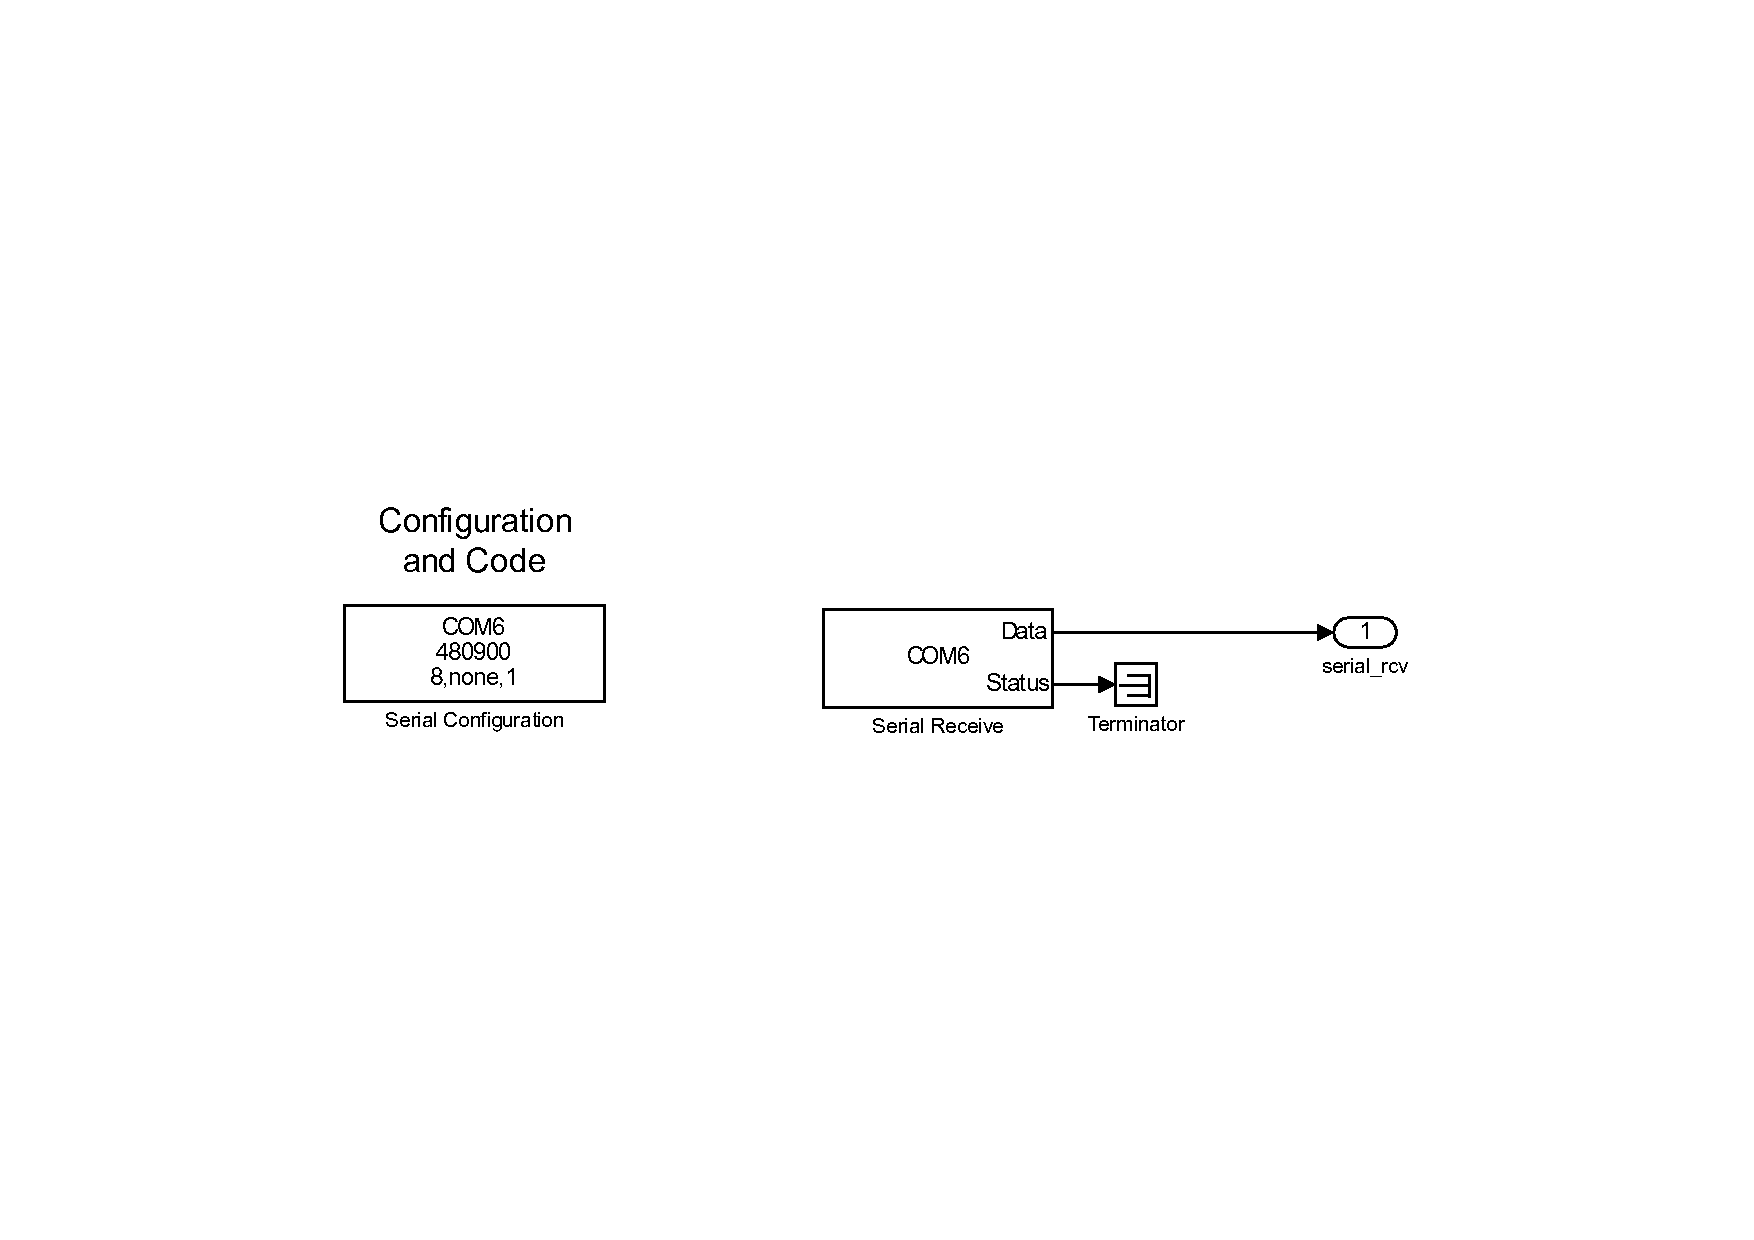
\includegraphics[scale=0.6, trim={5cm 8.5cm 5.5cm 8.5cm},clip]{pic/70_eigene_app/Serial_output.pdf}
  \caption{Serielle Schnittstelle}
  \label{fig:sub_sim_system}
  \end{center}
\end{figure}

\noindent
Die Pakete werden im System verarbeitet. Dazu wird eine 'Interpreted MATLAB Function' verwendet. Dieser Block unterstützt nur das double Format. Aus diesem Grund wurde ein Datentyp Konverter hinzugefügt. Der Parser liefert ein Vektor, welcher mit einem Demultiplexer die Kanäle separiert.
 \begin{figure}[ht]
  \begin{center}
  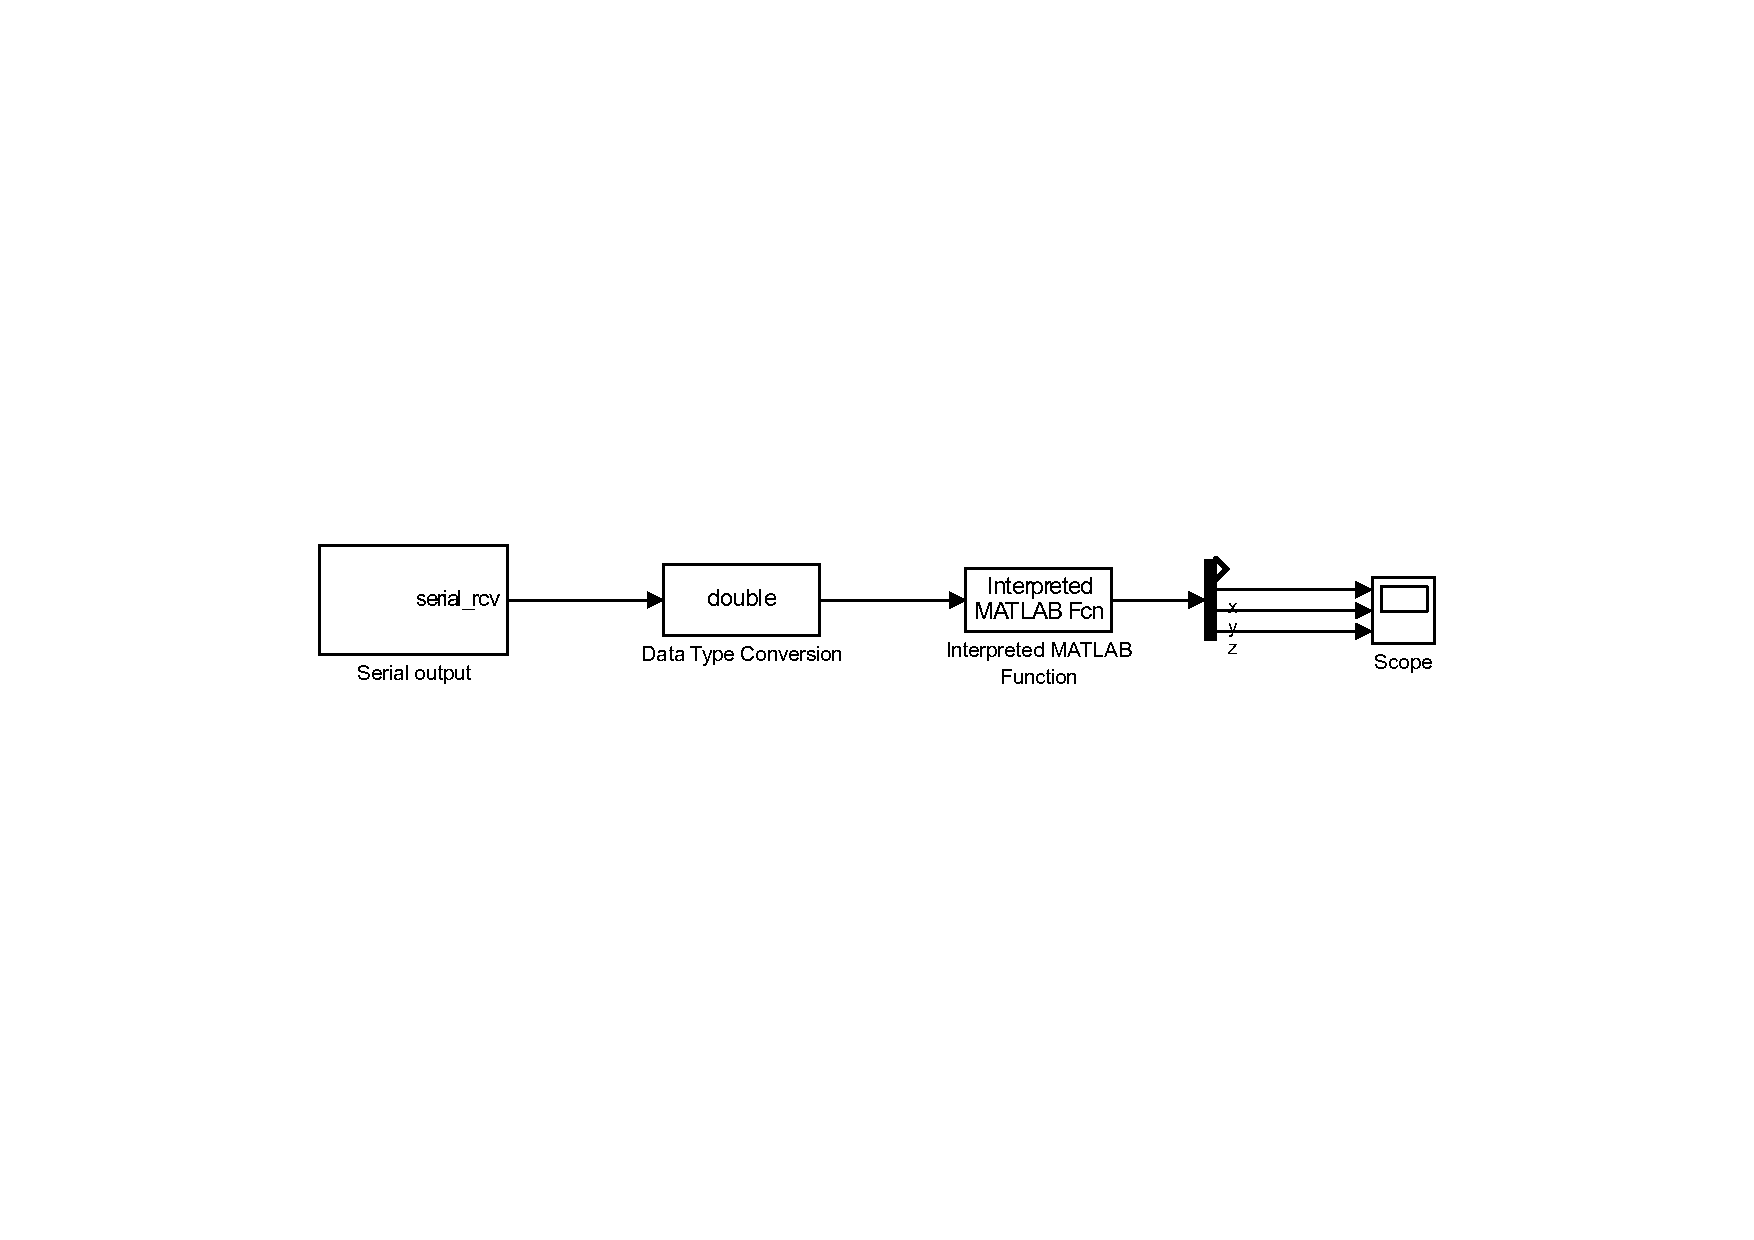
\includegraphics[scale=0.6, trim={5cm 9cm 4.8cm 8.5cm},clip]{pic/70_eigene_app/sys_main.pdf}
  \caption{Serielle Schnittstelle}
  \label{fig:main_sim_system}
  \end{center}
\end{figure}

\noindent
In der Abbildung \ref{fig:accel_looping} ist der Scope ersichtlich. Auf der x-Achse befindet sich die Zeit in Sekunden. Die y-Achse beschreibt die Beschleunigung in x, y und z-Richtung in $\frac{m}{s^2}$.  Der Scope kann während der Simulation geöffnet werden und zeigt die Daten zur Laufzeit an.
\begin{figure}[ht]
  \begin{center}
  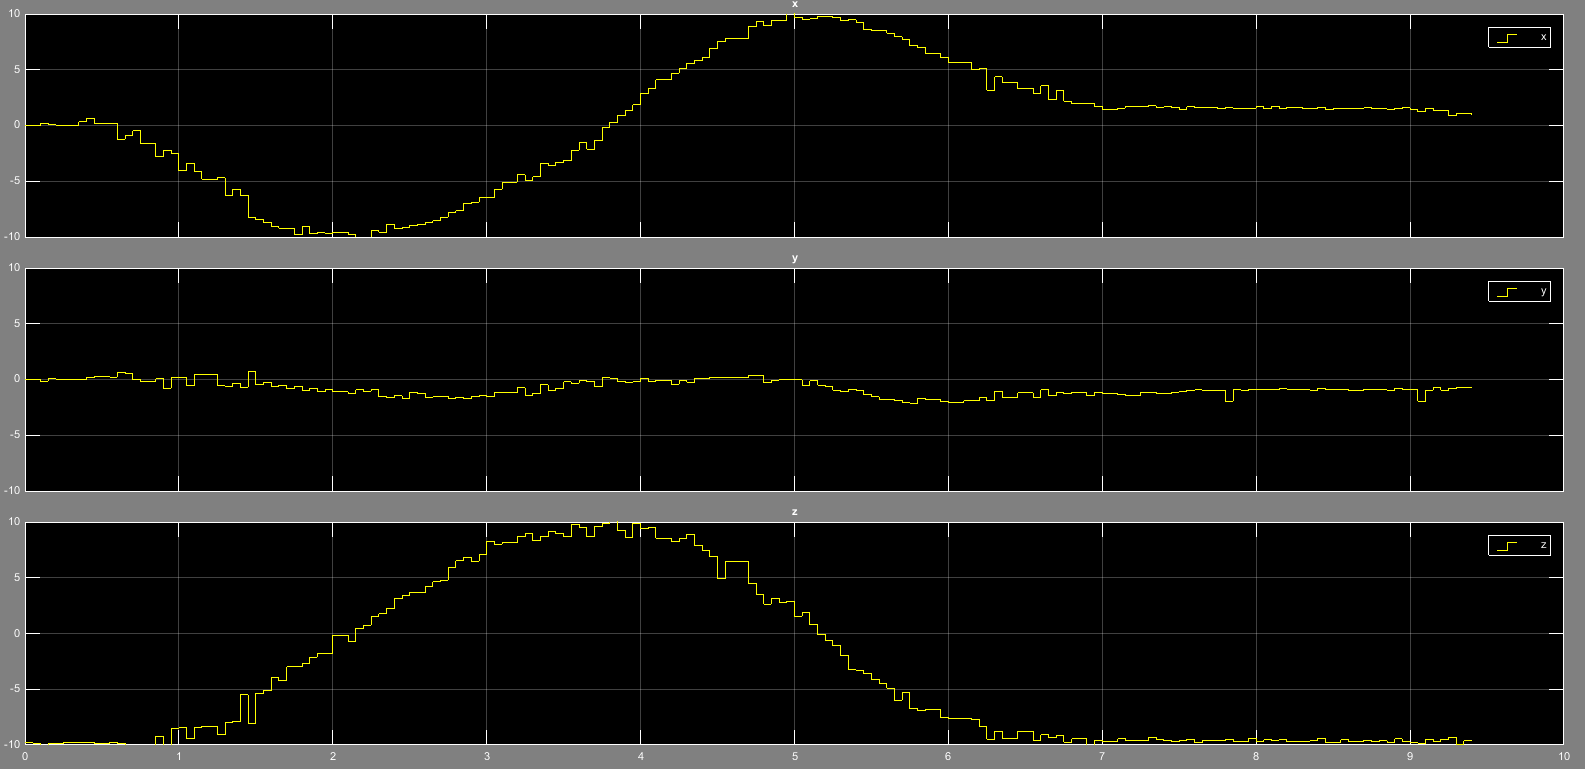
\includegraphics[scale=0.3]{pic/70_eigene_app/looping.png}
  \caption{Accelorometer während eines Looping}
  \label{fig:accel_looping}
  \end{center}
\end{figure}






\clearpage
